%!TEX TS-program = Arara
% arara: pdflatex: {shell: yes}
% arara: pdflatex: {shell: yes}
\documentclass[12pt,ngerman,parskip=half,oneside,openany]{scrbook}
% oneside => Dokument soll einseitig gedruckt werden
% openany => neue Kapitel etc. dürfen auf jeder Seite anfangen

\usepackage{booktabs} % schöne Tabellen
\usepackage{babel} % eindeutschen
\usepackage{graphicx} % Grafiken einfügen
\usepackage{csquotes} % Text in Gänsefüßchen
\usepackage{paralist} % kompakte Aufzählungen
\usepackage{xcolor} % Farben


\usepackage{hyperref} % klickbare Links, als letztes laden
\hypersetup{
    bookmarks=true,                     % show bookmarks bar
    unicode=false,                      % non - Latin characters in Acrobat’s bookmarks
    pdftoolbar=true,                        % show Acrobat’s toolbar
    pdfmenubar=true,                        % show Acrobat’s menu
    pdffitwindow=false,                 % window fit to page when opened
    pdfstartview={FitH},                    % fits the width of the page to the window
    pdftitle={Dissertation},                        % title
    pdfauthor={Donald Duck},                 % author
    pdfsubject={Raketen},                   % subject of the document
    pdfcreator={Donald Duck},                   % creator of the document
    pdfproducer={LaTeX},             % producer of the document
    pdfkeywords={Rockets, Fuel},   % list of keywords
    pdfnewwindow=true,                  % links in new window
    colorlinks=true,                        % false: boxed links; true: colored links
    linkcolor=blue,                          % color of internal links
    filecolor=blue,                     % color of file links
    citecolor=blue,                     % color of file links
    urlcolor=blue                        % color of external links
}


%\usepackage[math]{iwona}
%\usepackage{arev}
%\usepackage{fouriernc}
%\usepackage{concmath} % Nicht benutzen
\usepackage[math]{kurier}
\usepackage[T1]{fontenc}

\usepackage[pagewise]{lineno}
\linenumbers

\usepackage{blindtext}
% Wenn man nur einzelne Kapitel übersetzen möchte,
% die Seitenzahlen aber korrekt sein sollen.
%\includeonly{Analyse,Fazit}

\begin{document}

\AddToShipoutPicture*{\put(400,750){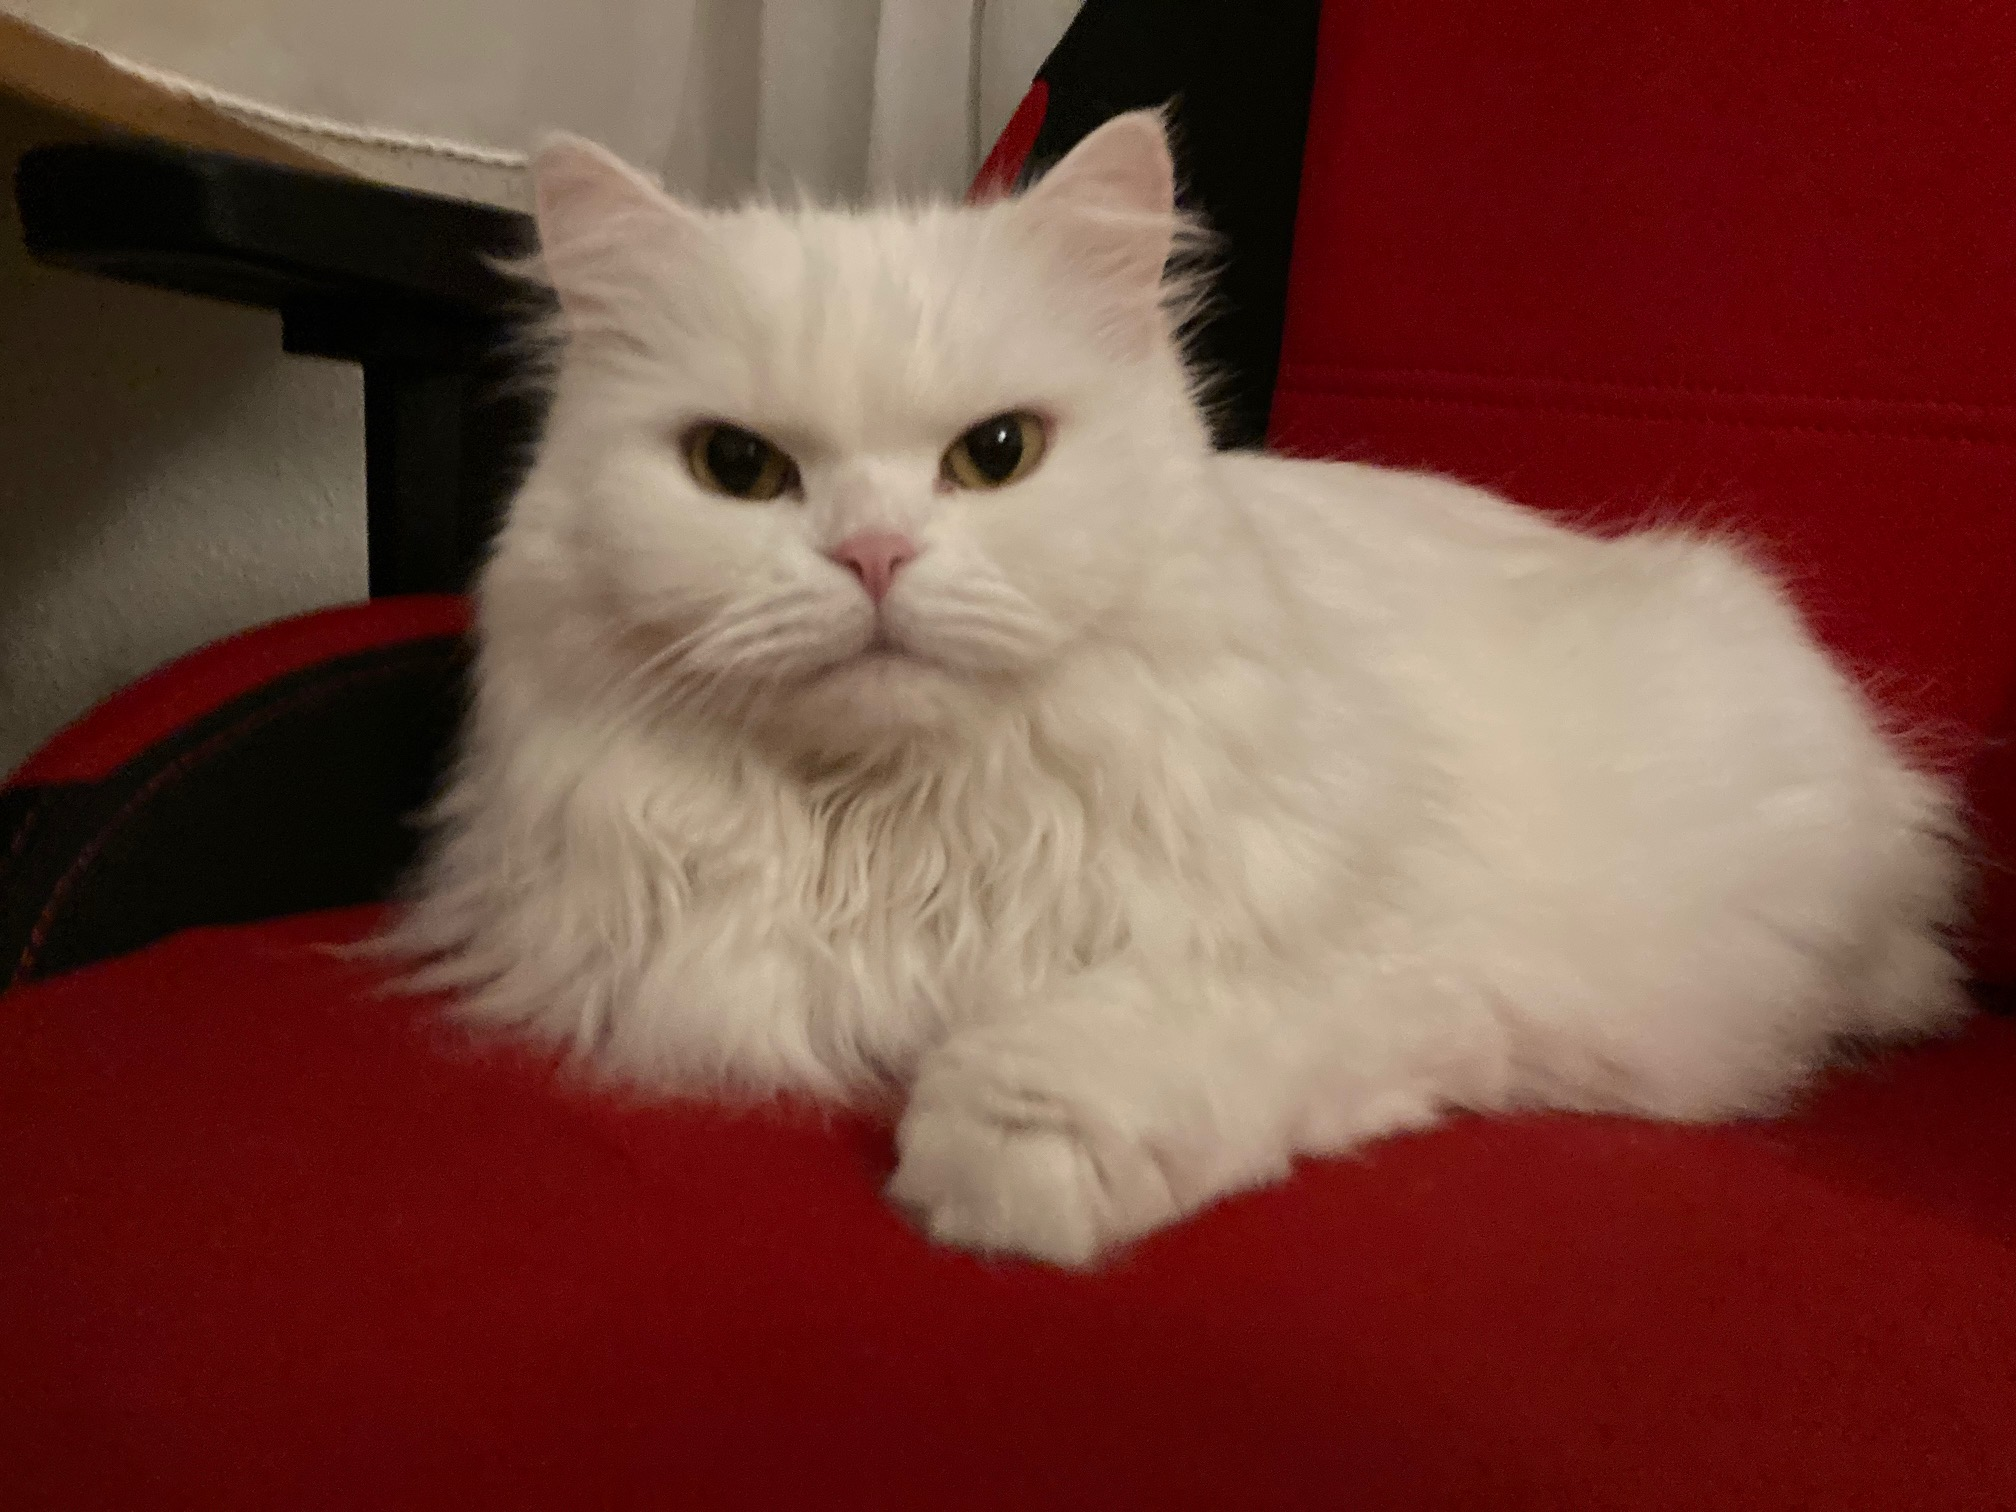
\includegraphics[width=3cm]{Bilder/Katze}}}

\begin{titlepage}
{\bfseries\Large Technische Universität Entenhausen \\ Fakultät für Raketentechnik \\ Lehrstuhl Quantenraketen}\vspace*{3cm}

\begin{center}
\LARGE\bfseries\enquote{Albert Einstein, Genie und Raketen}
\end{center}\vspace*{2cm}

\begin{center}
\LARGE\bfseries Dissertation\\ zur Erlangung des Titels\\ Dr. ing. \\ von \\ Donald Duck
\end{center}



%\vfill % fülle die Seite aber lass Platz für
%{\large Betreuer: Prof. Dr. Daniel Düsentrieb \\ 
%Zweitgutachter: Dagobert Duck \\
%Köln, den 01.01.2026}
%
%\hfill Version vom \today
\vfill
\begin{tabular}{p{0.49\textwidth}l}
\bfseries\large Betreuer: & \bfseries\large  Prof. Dr. Daniel Düsentrieb \\
\bfseries\large Zweitgutachter: & \bfseries\large  Dagobert Duck \\
\end{tabular}

\end{titlepage}

\frontmatter
\tableofcontents

\listoffigures

\listoftables

\mainmatter

%!TeX root = Dissertation-DonaldDuck.tex
\chapter{Einleitung}\label{cha:Einleitung}

\blindtext[5]

\begin{figure}
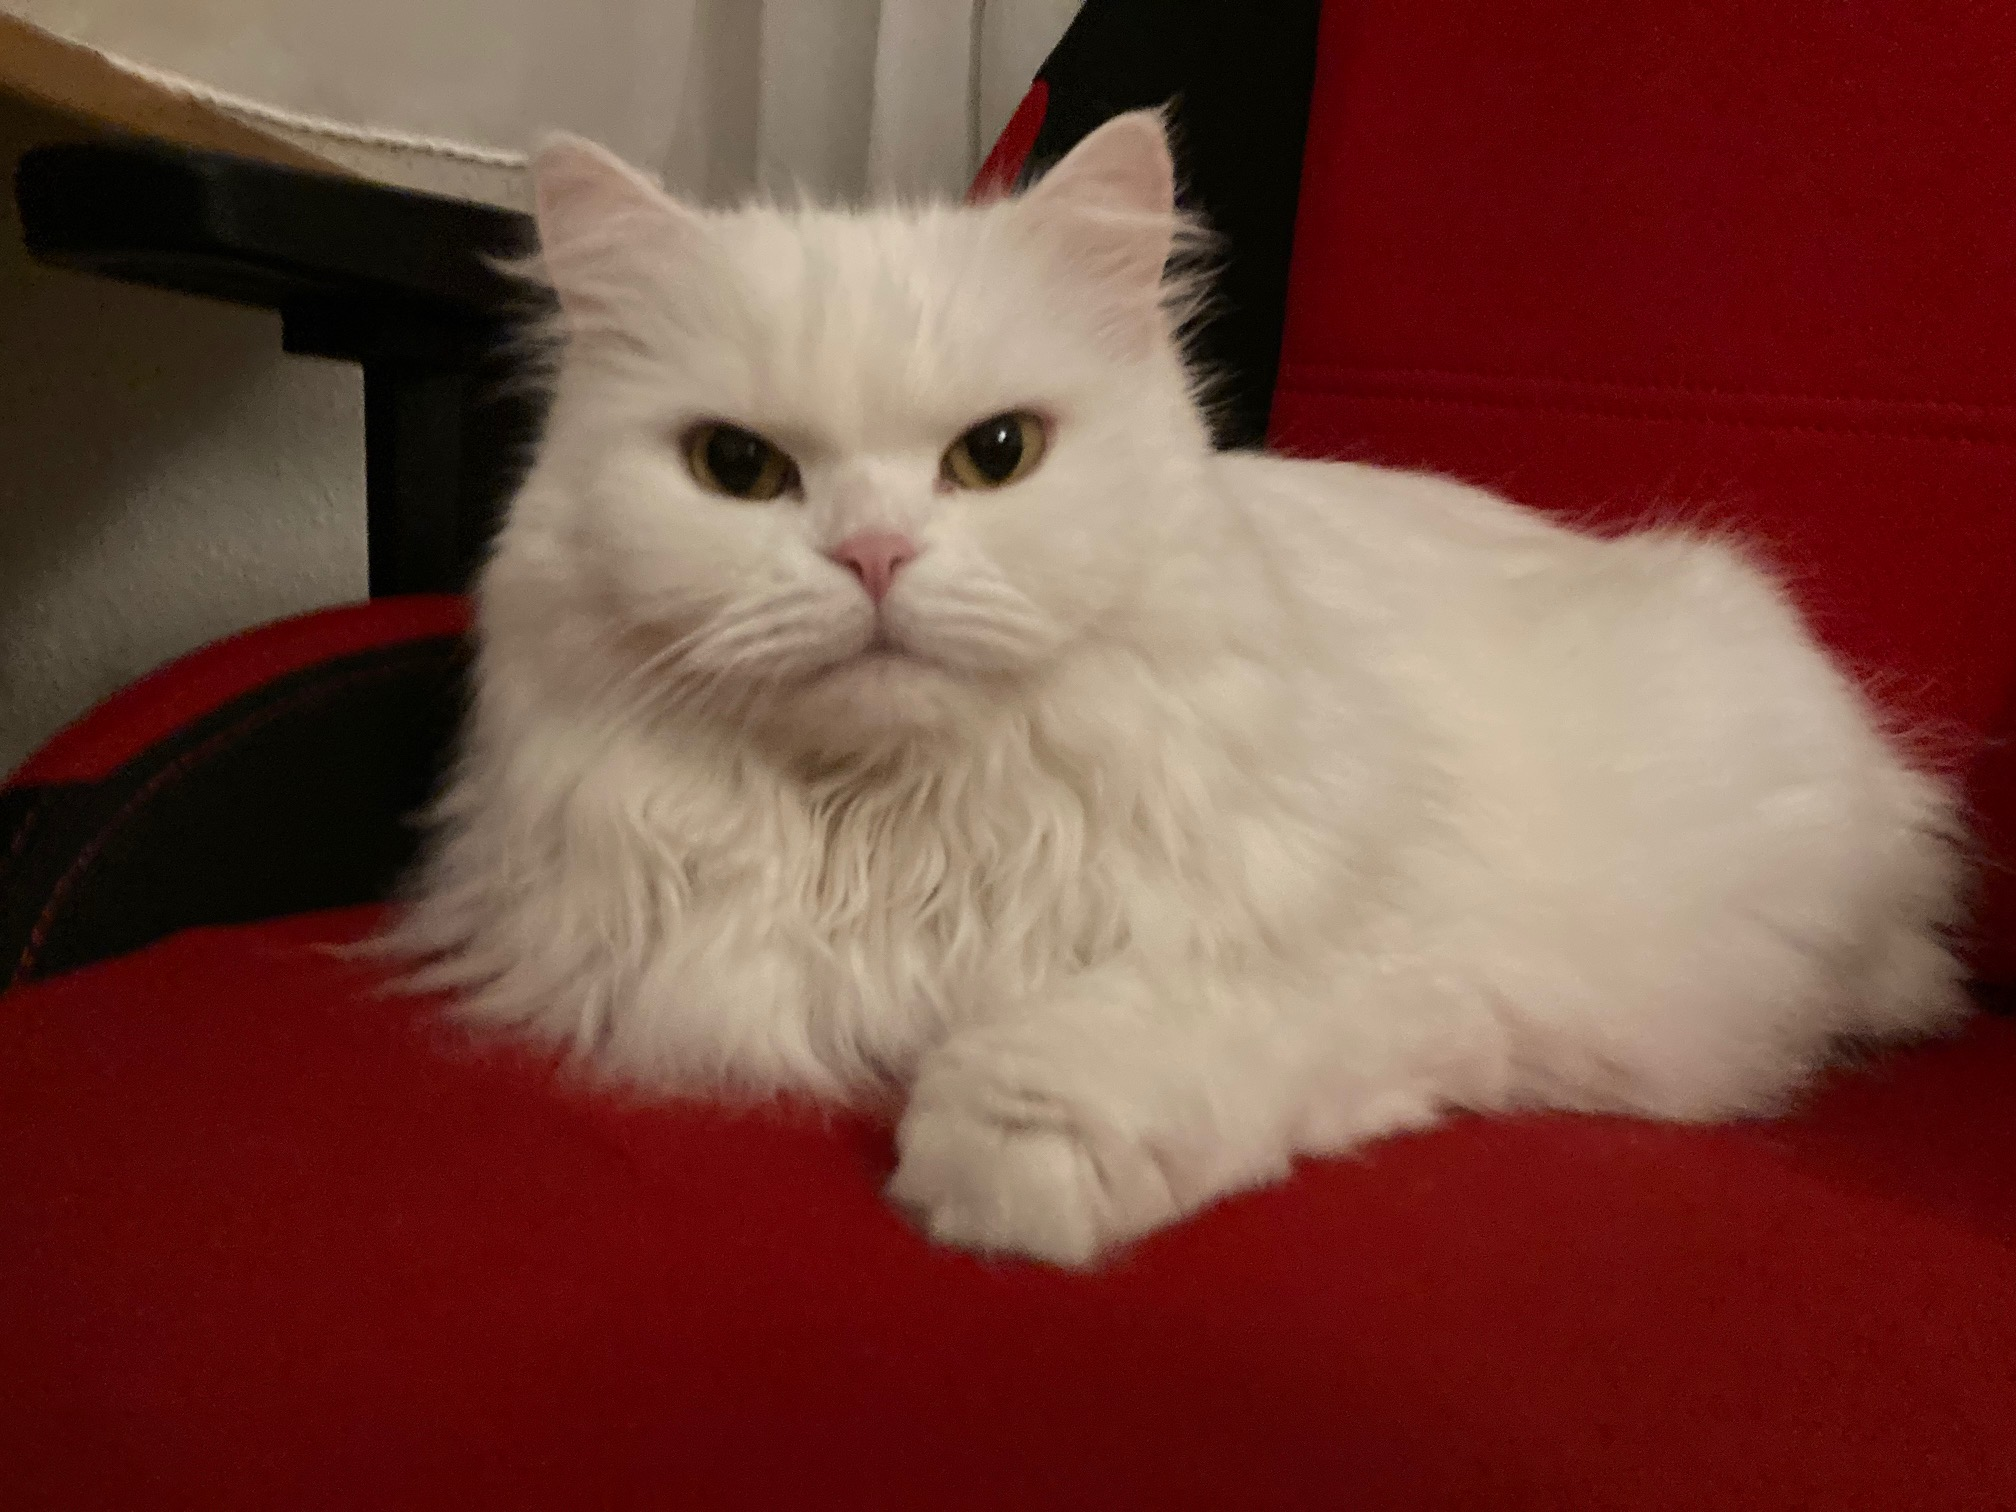
\includegraphics[width=\textwidth]{Bilder/Katze}
\caption{Meine Katze}\label{fig:Katze}
\end{figure}

\blindtext[5]

% Alternative zum Float
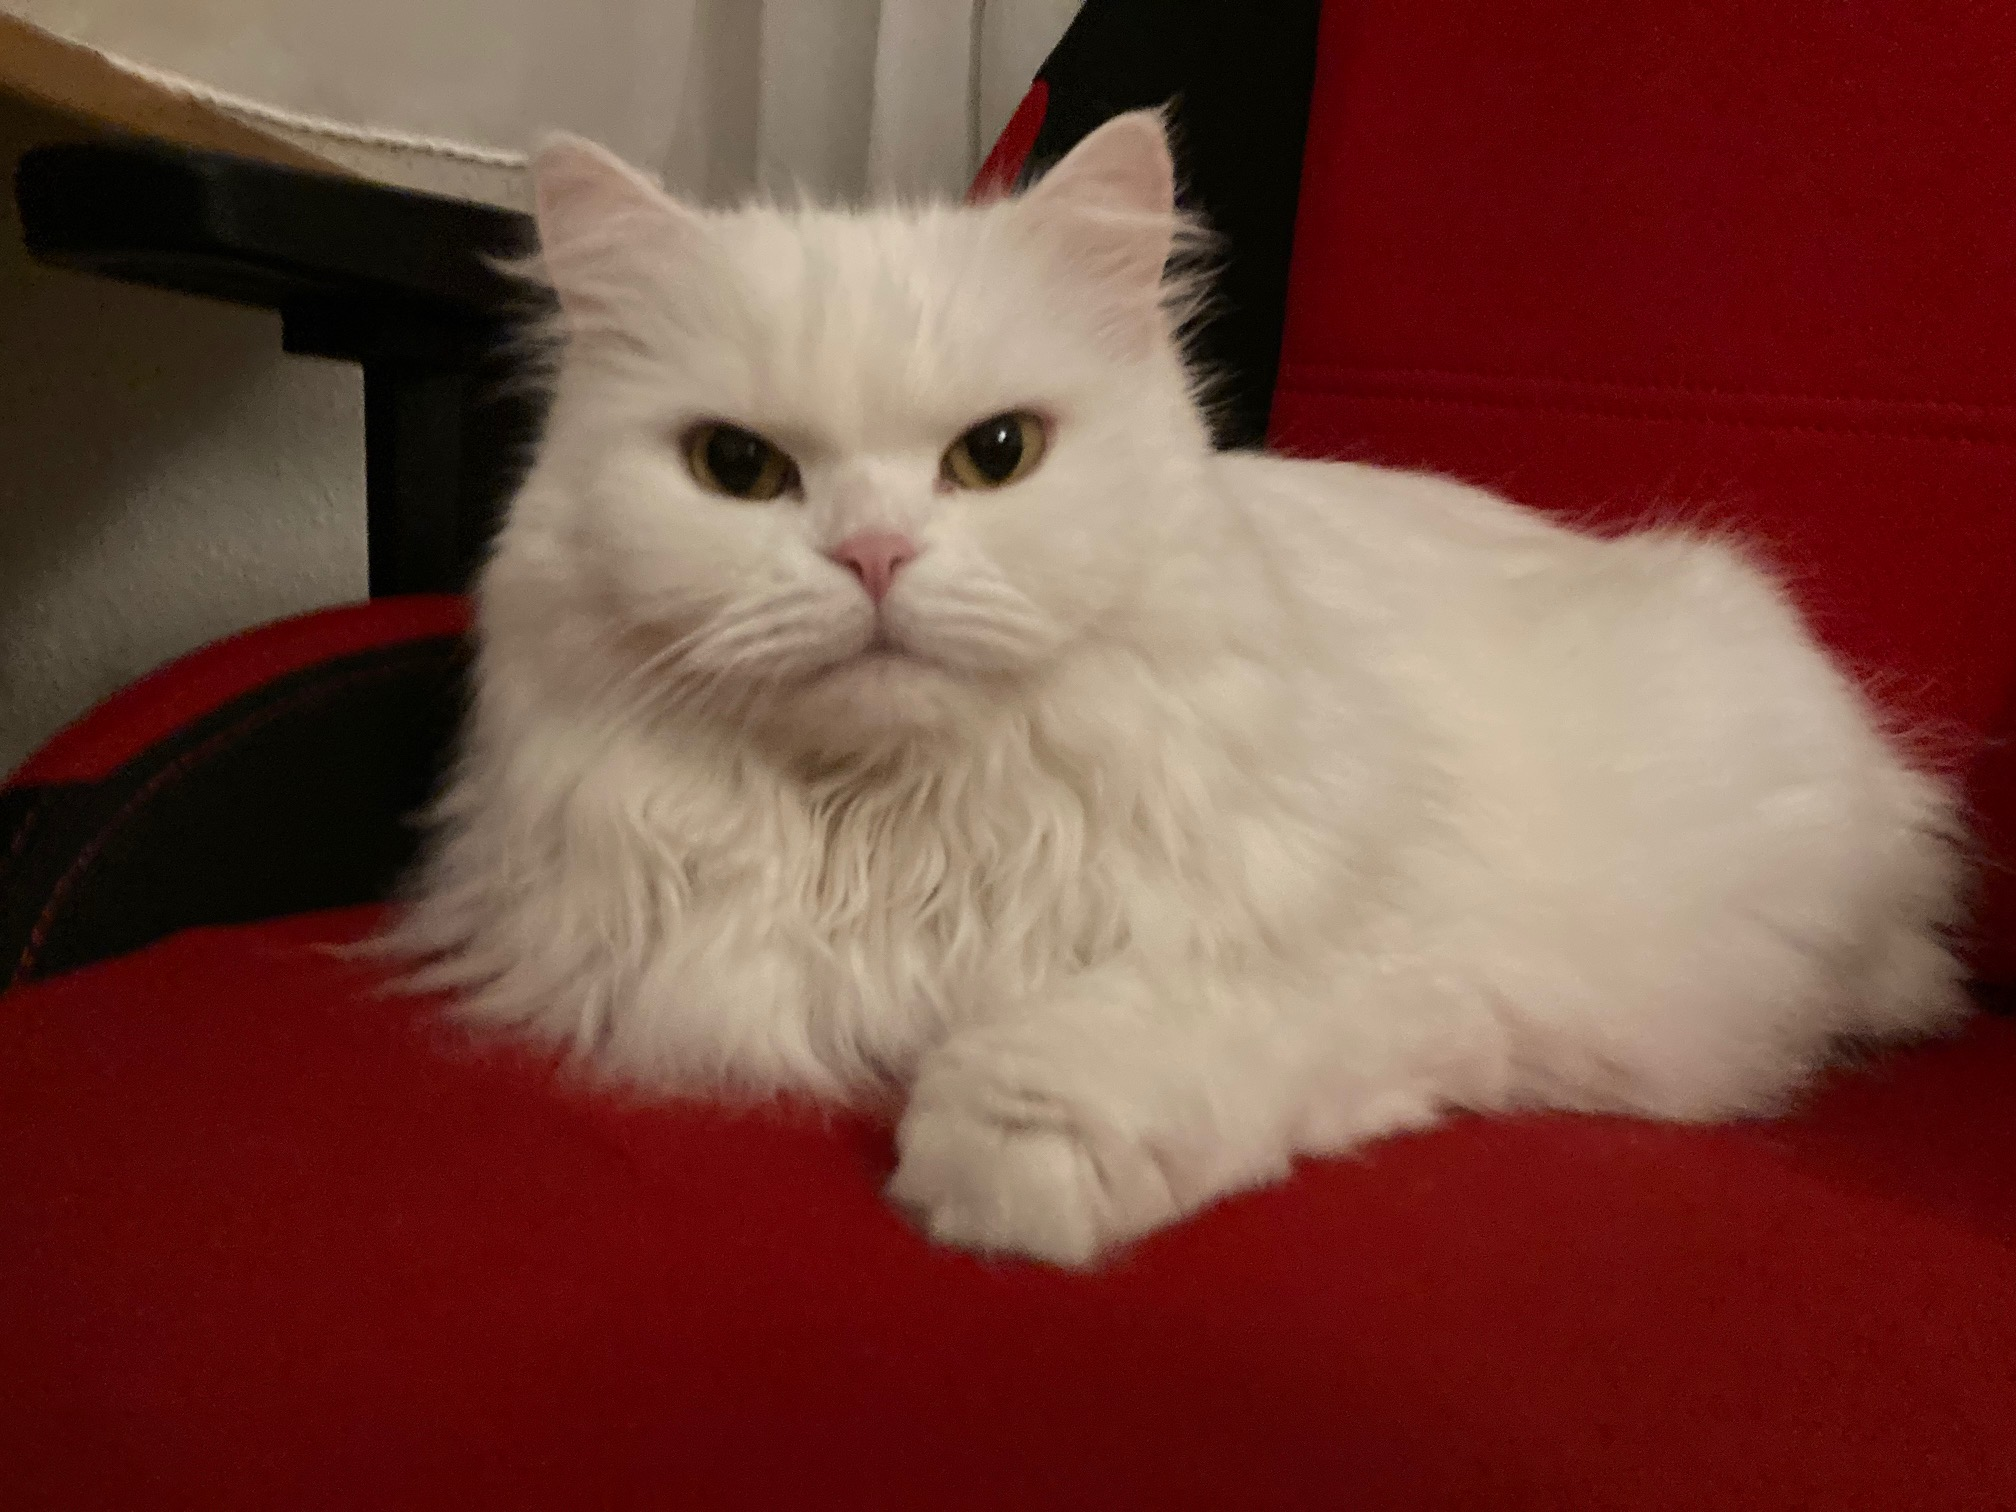
\includegraphics[width=\textwidth]{Bilder/Katze}
\captionof{figure}{Meine Katze 2}\label{fig:Katze2}

\blindtext[12]

\begin{equation}\label{eq:pythagoras}
-\frac{p}{2} \pm \sqrt{ \left(\frac{p}{2}\right)^2 -q }
\end{equation}

\begin{equation}\label{eq:pythagoras}
-\frac{p}{2} \pm \sqrt{ \left(\frac{p}{2}\right)^2 -q }
\end{equation}

\begin{equation}\label{eq:pythagoras}
-\frac{p}{2} \pm \sqrt{ \left(\frac{p}{2}\right)^2 -q }
\end{equation}


\begin{equation}
\sum_{i=1}^{\infty} \sqrt[2\,]{i\times \prod_{x=\sum_{i=1}^{\infty}} \pi \cdot \alpha \beta \gamma 
\frac{\frac{1}{2}}{\frac{3}{4}}
}
\end{equation}

\$

%!TeX root = Dissertation-DonaldDuck.tex
\chapter{Analyse}\label{cha:Analyse}

\blindtext[5]

\begin{figure}
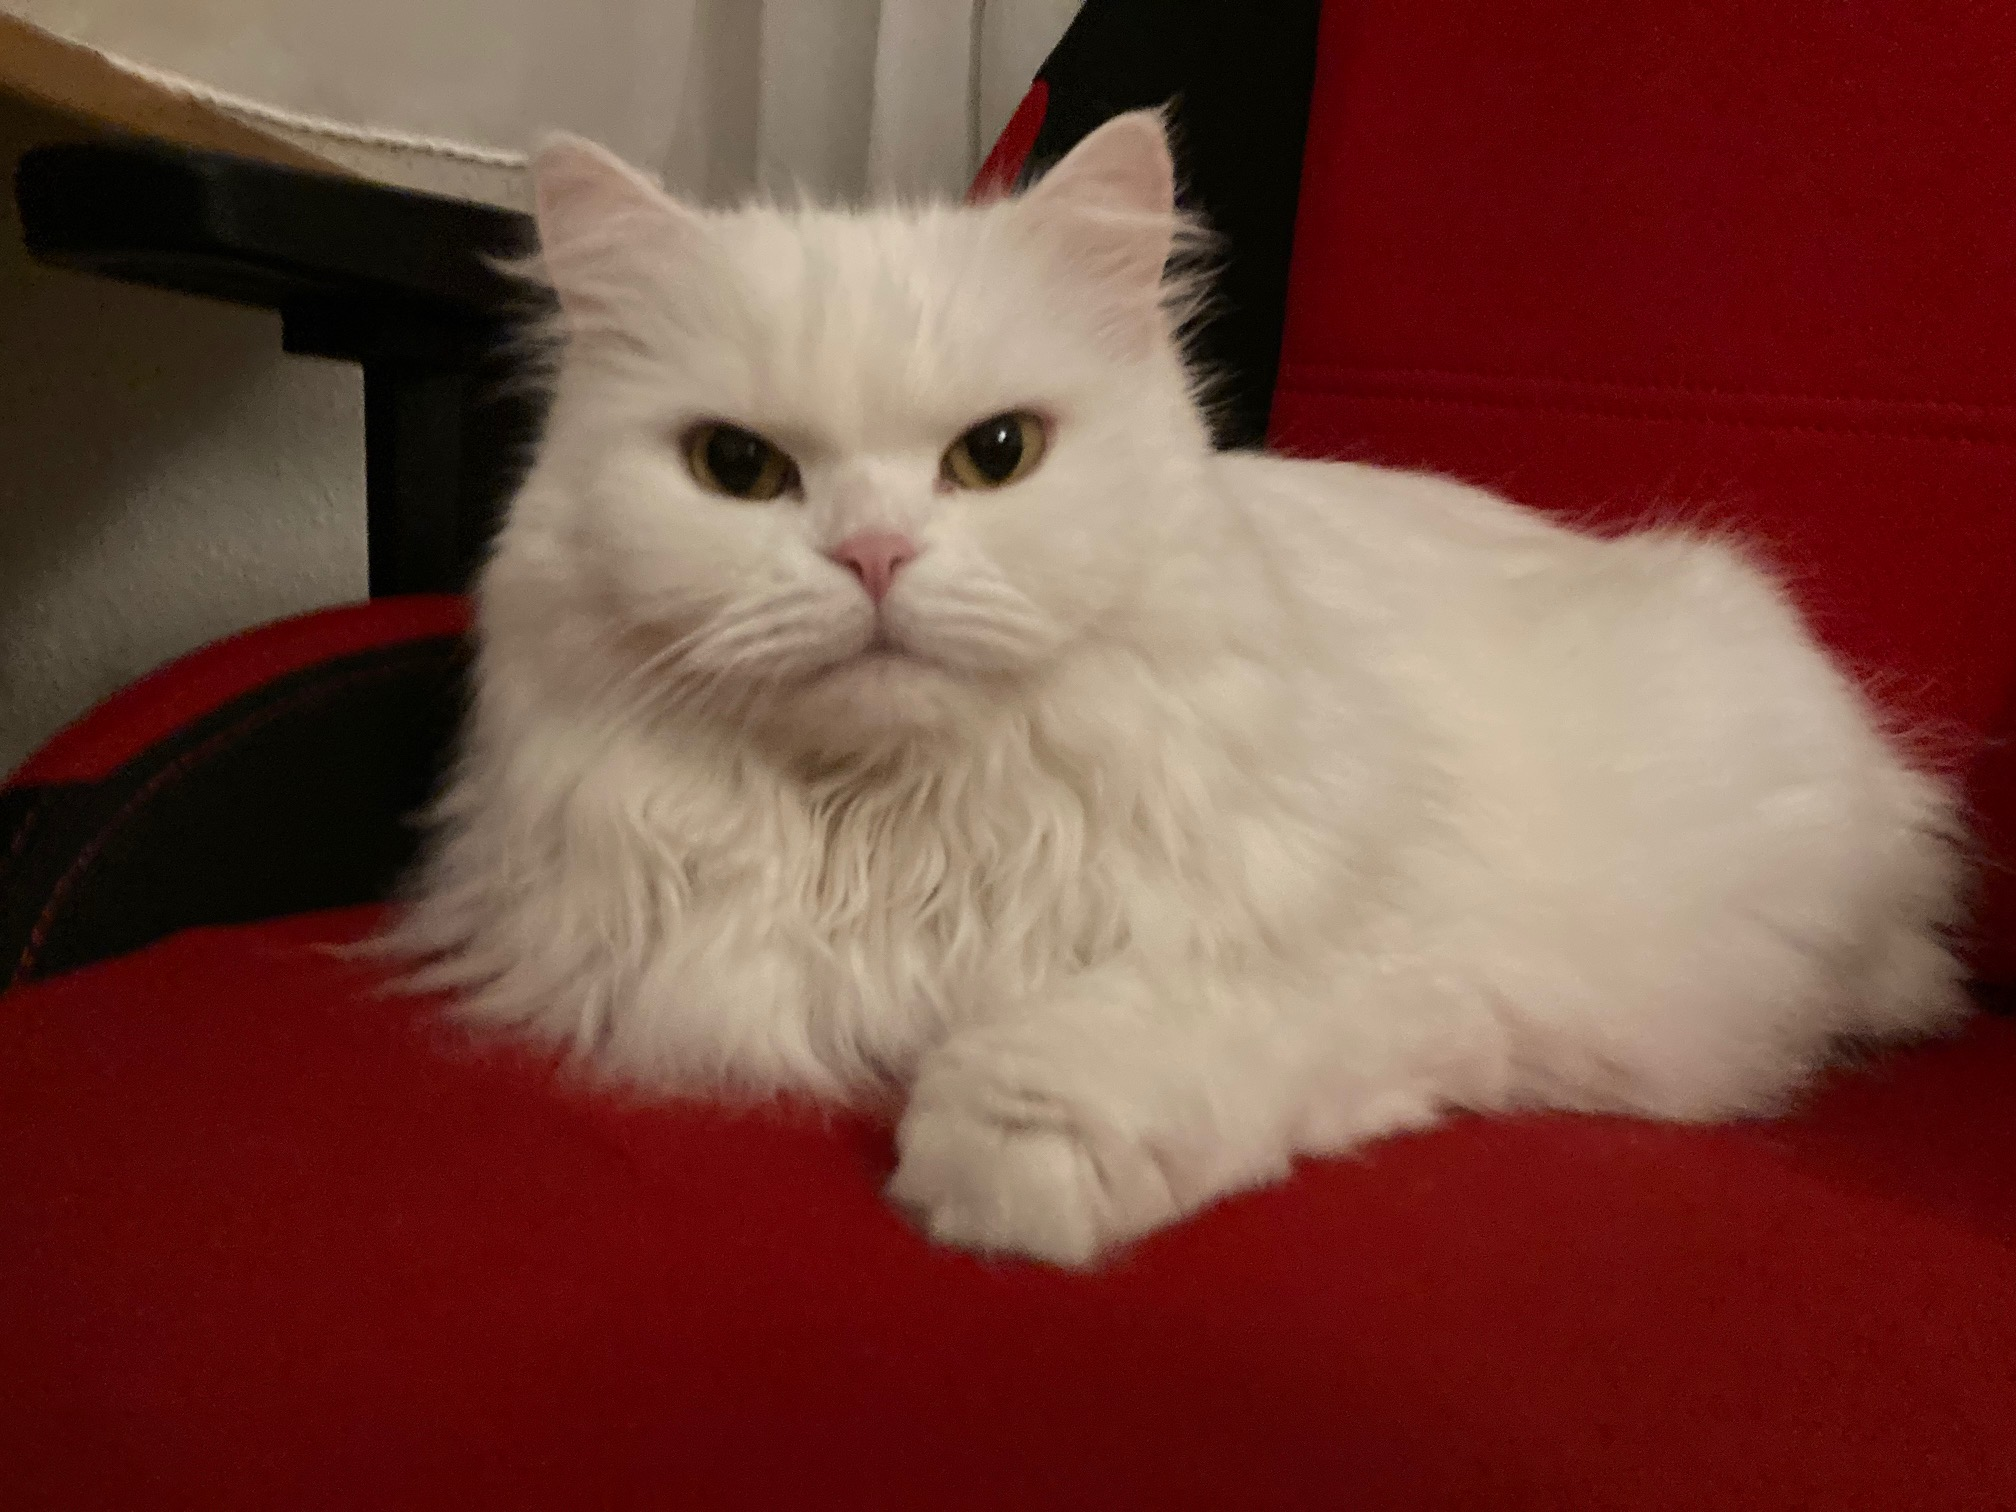
\includegraphics[width=\textwidth]{Bilder/Katze}
\caption{Meine Katze}\label{fig:Katze}
\end{figure}

\blindtext[5]

% Alternative zum Float
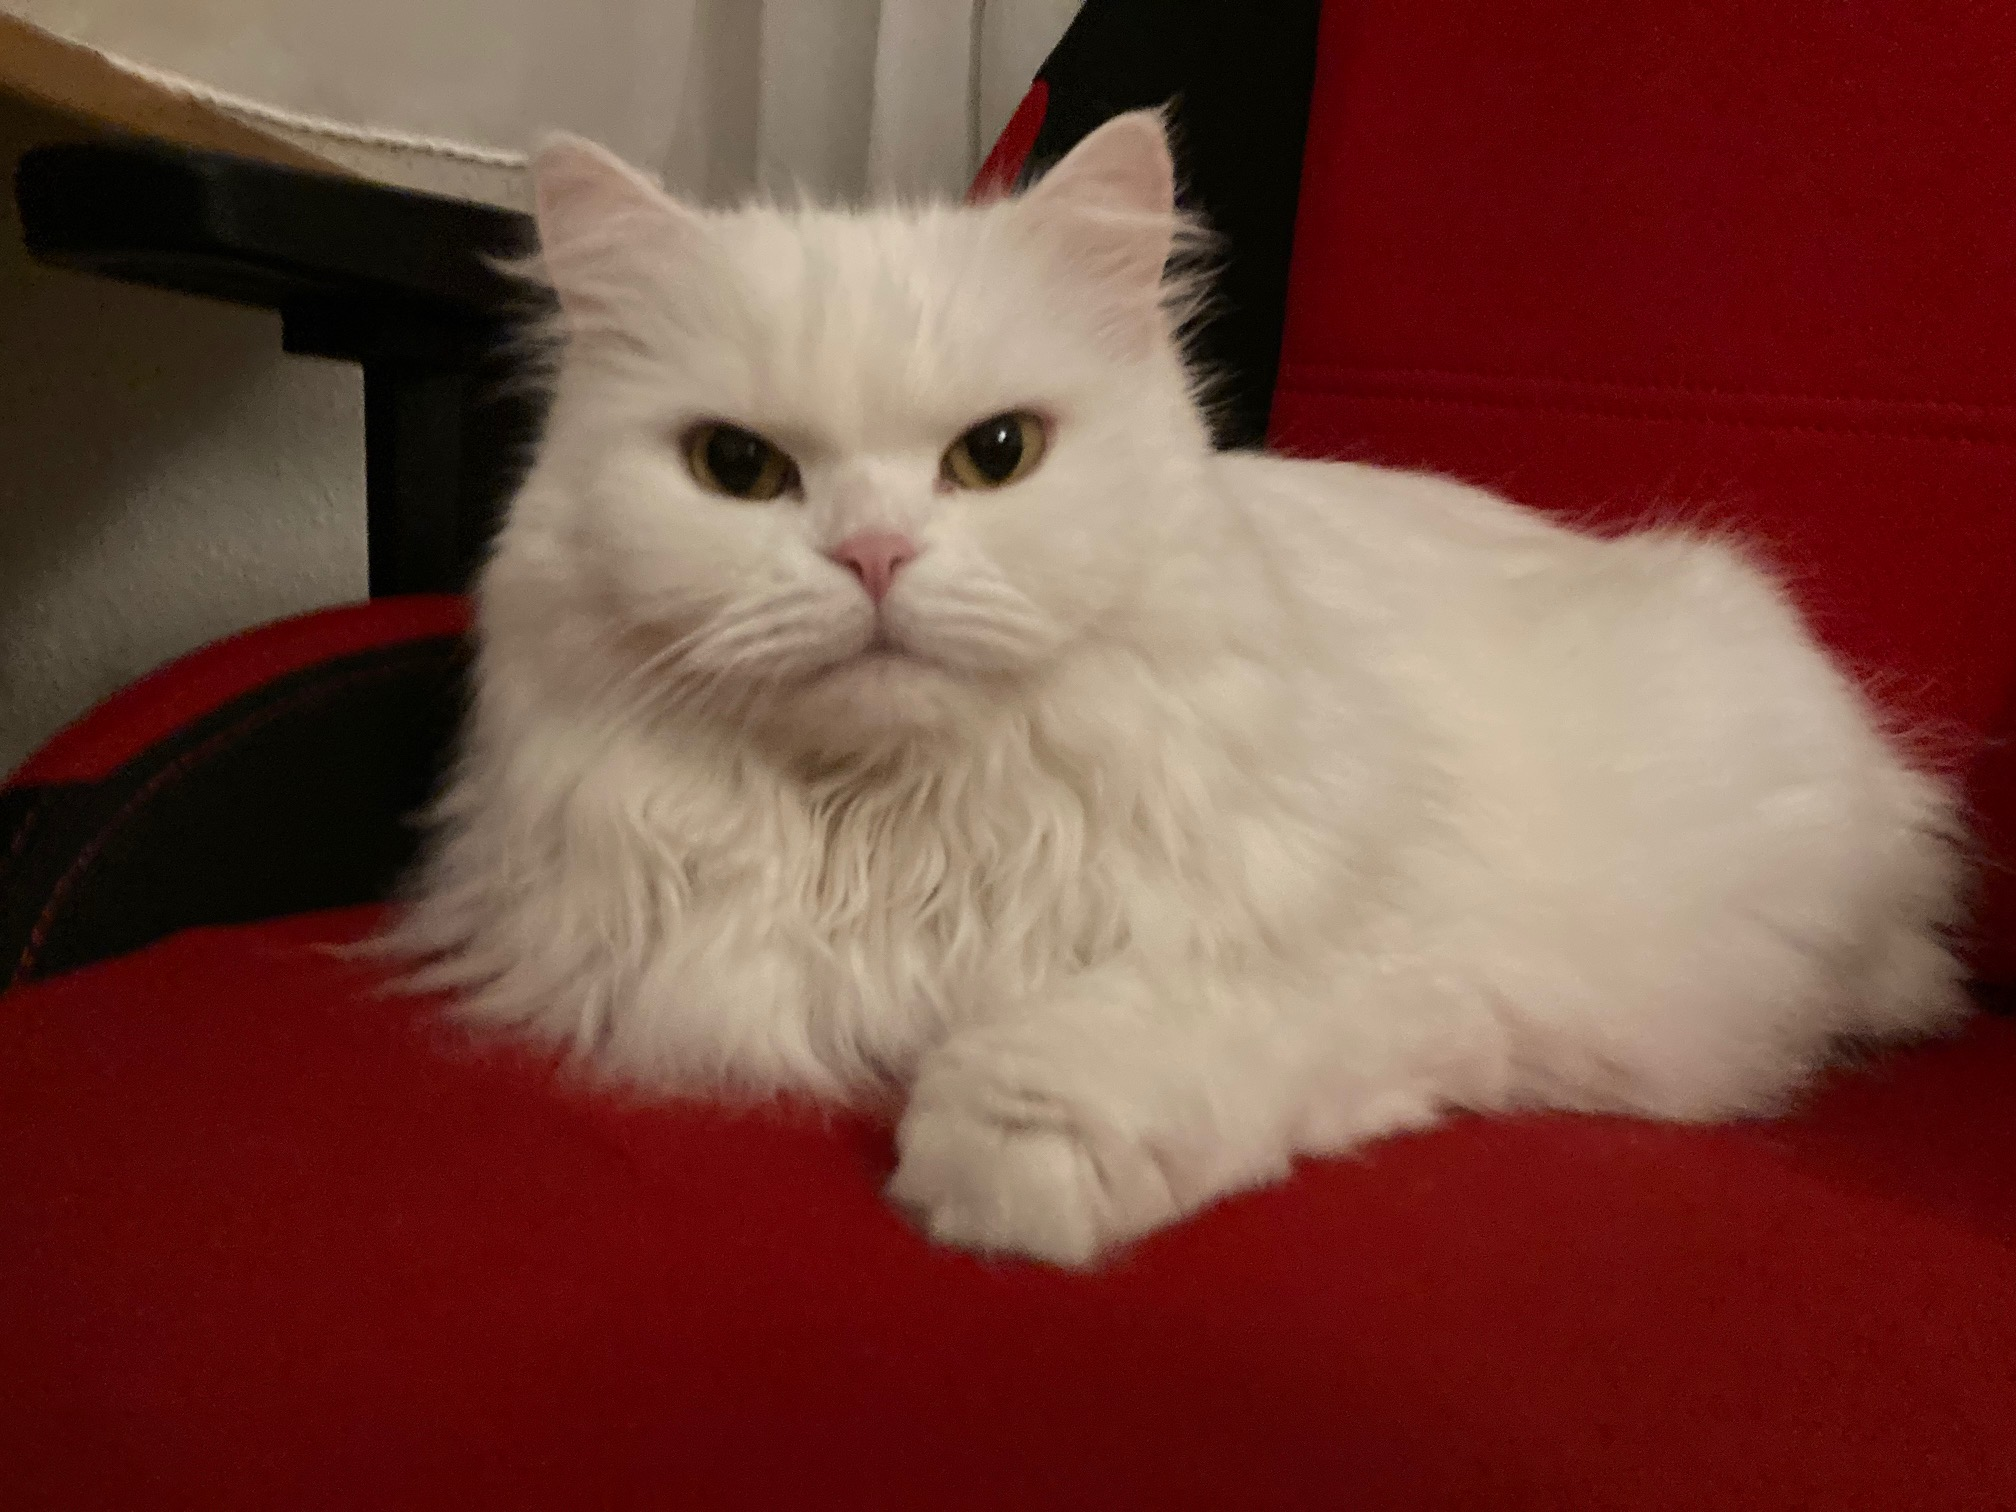
\includegraphics[width=\textwidth]{Bilder/Katze}
\captionof{figure}{Meine Katze 2}\label{fig:Katze2}

\blindtext[12]

\blindtext[12]

\blindtext[12]

\blindtext[12]

%!TeX root = Dissertation-DonaldDuck.tex
%!TEX TS-program = Arara
% arara: pdflatex: {shell: yes}
% arara: pdflatex: {shell: yes}
\chapter{Fazit}\label{cha:Fazit}

\blindtext[5]

\begin{figure}
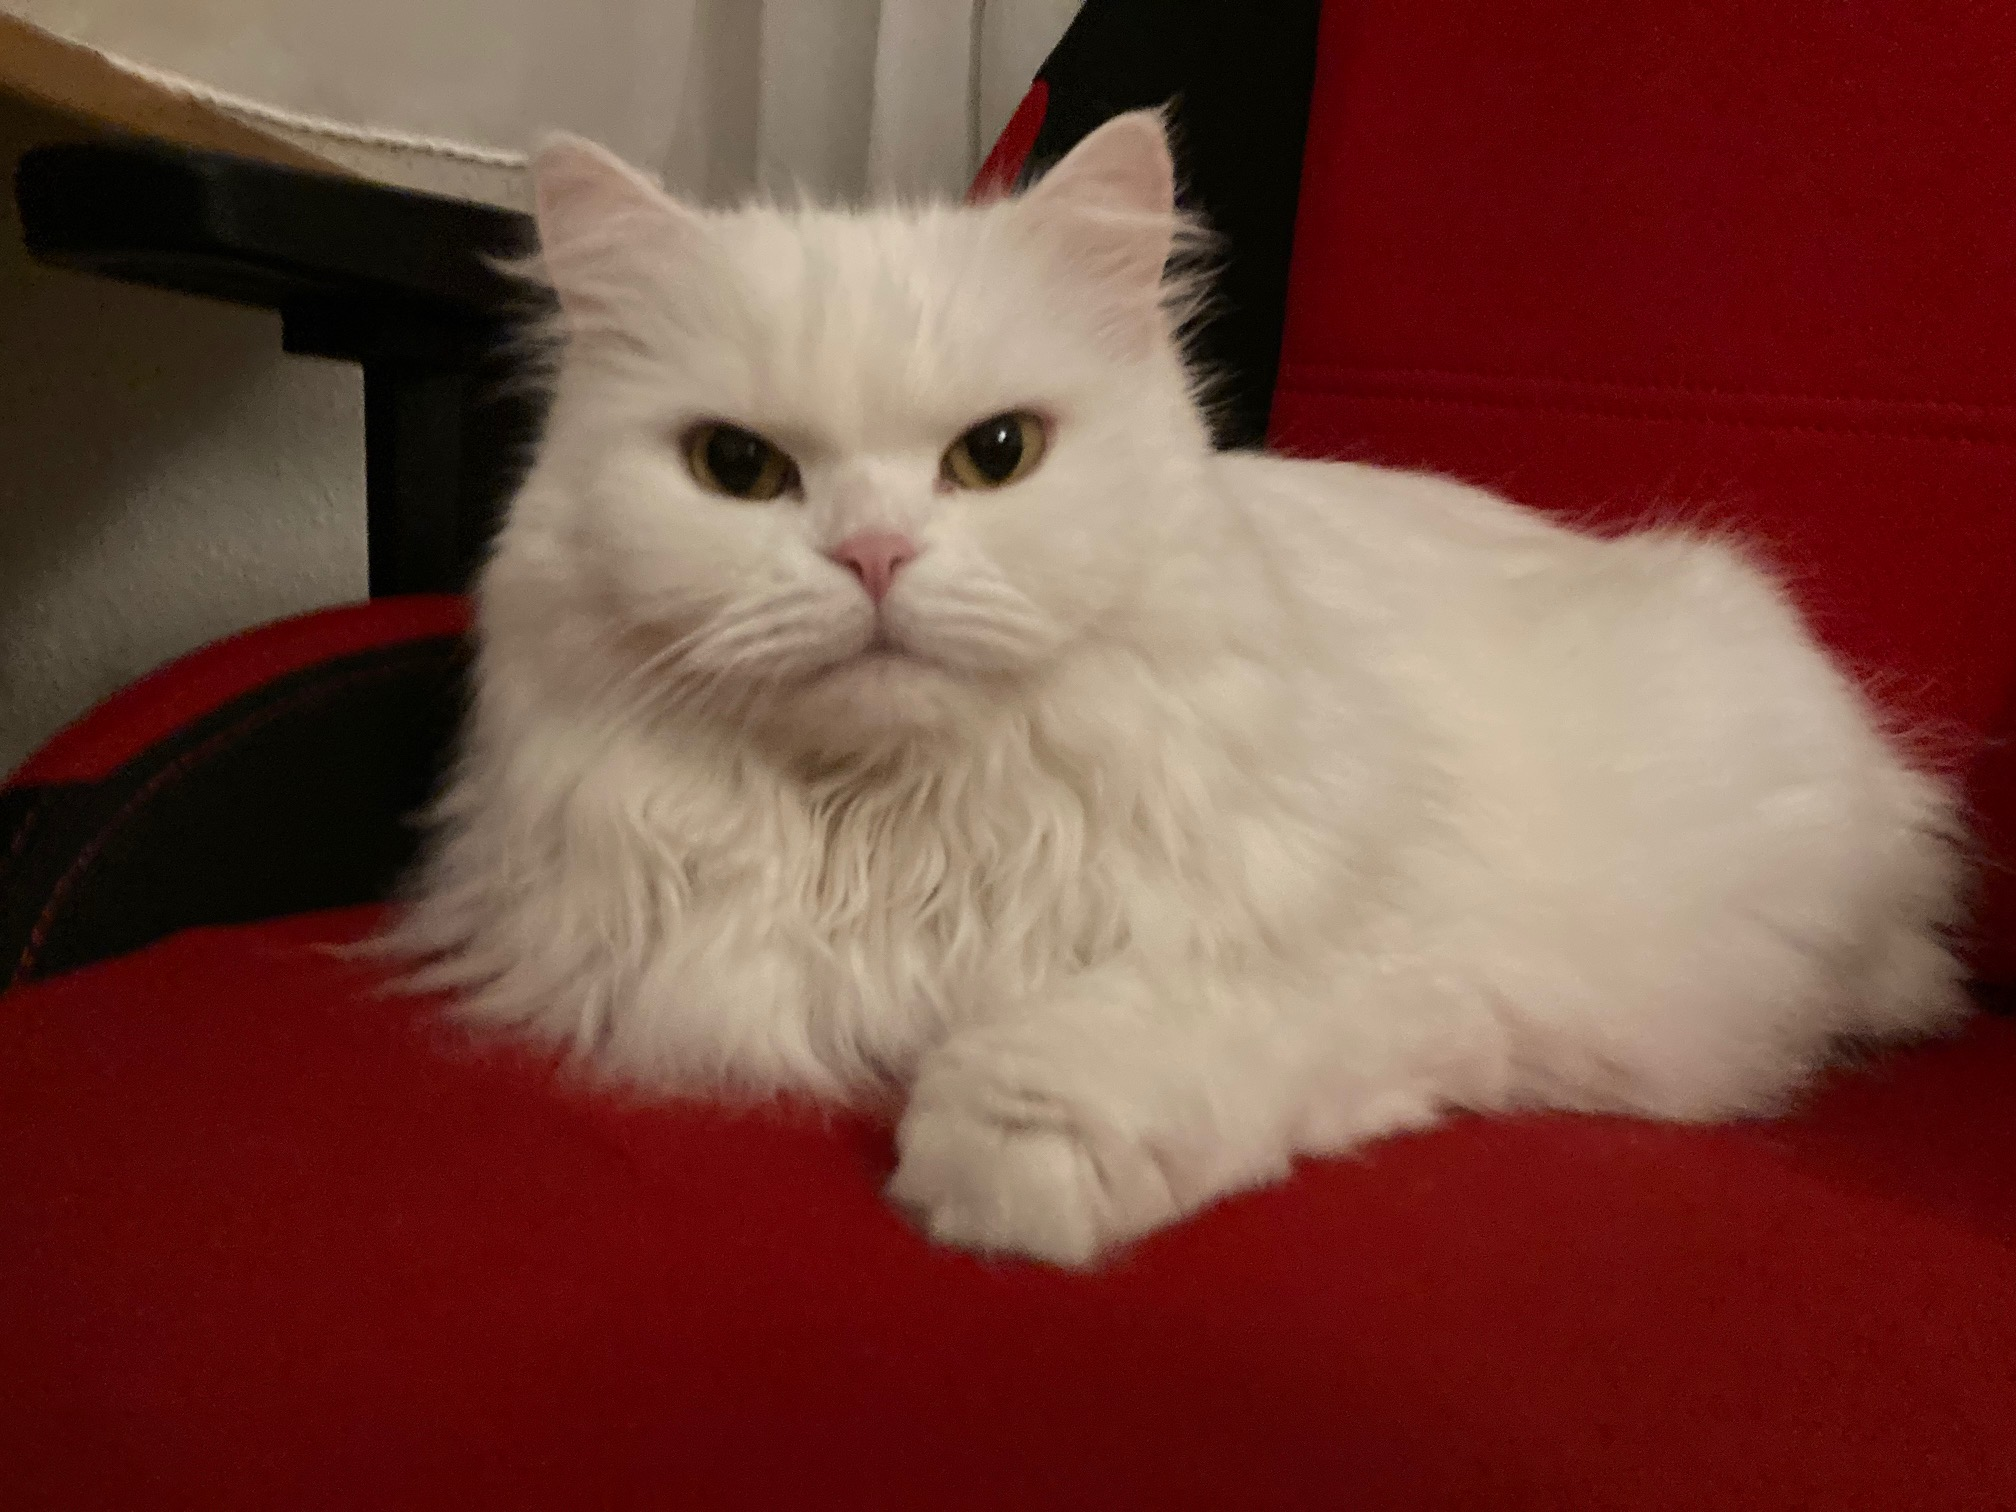
\includegraphics[width=\textwidth]{Bilder/Katze}
\caption{Meine Katze}\label{fig:Katze}
\end{figure}

\blindtext[5]

% Alternative zum Float
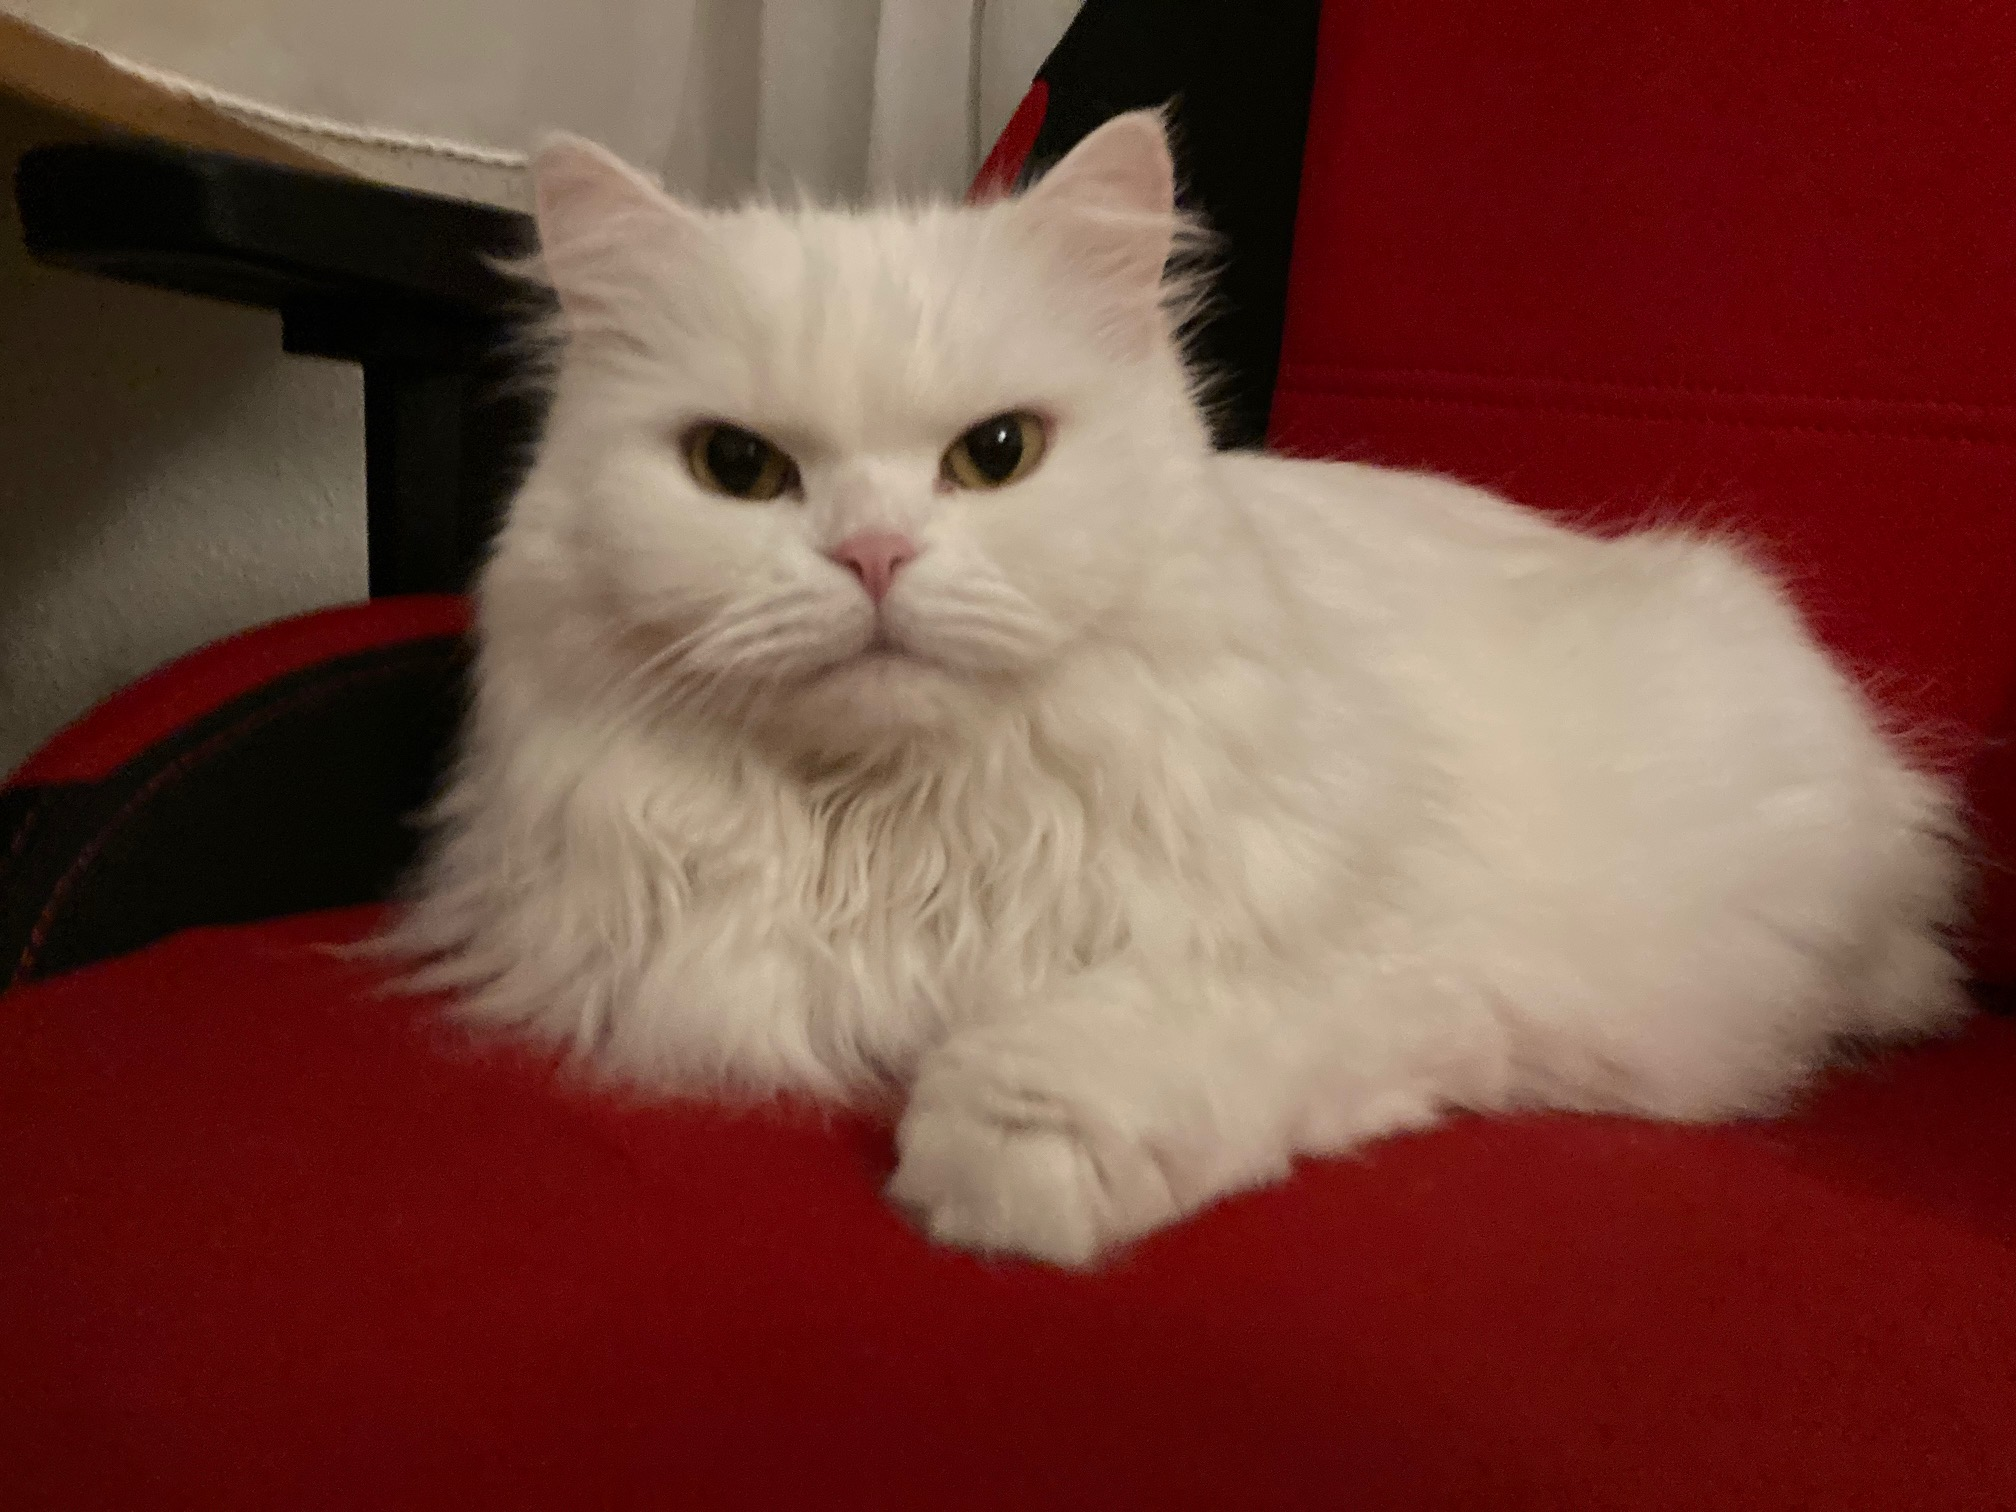
\includegraphics[width=\textwidth]{Bilder/Katze}
\captionof{figure}{Meine Katze 2}\label{fig:Katze2}

\blindtext[12]

\blindtext \cite{Knuth1984}, \cite{Knuth1984}  and \cite{Buchin2023} have shown, that elliptic curves are useful in computing. \cite{Yu2021} also showed this   .\footnote{\blindtext}

\cite{Ziegenhagen2022}

parencite \parencite{Knuth1984}

Uwe Ziegenhagen\footcite{Ziegenhagen2022}

citeauthor, citetitle und citeyear kombiniert: \citeauthor{Knuth1984} hat in seinem im Jahre \citeyear{Knuth1984} erschienenen Buch \citetitle{Knuth1984} bewiesen, dass \(p = np \)

\printbibliography[title={Bücher},type=book] 

\printbibliography[title={Artikel},type=article] 

\printbibliography[title={Online-Quellen},type=www] 



\backmatter

%!TeX root = Dissertation-DonaldDuck.tex
\chapter{Anhang}\label{cha:Anhang}

\section{Bla}
\blindtext[5]

\begin{figure}
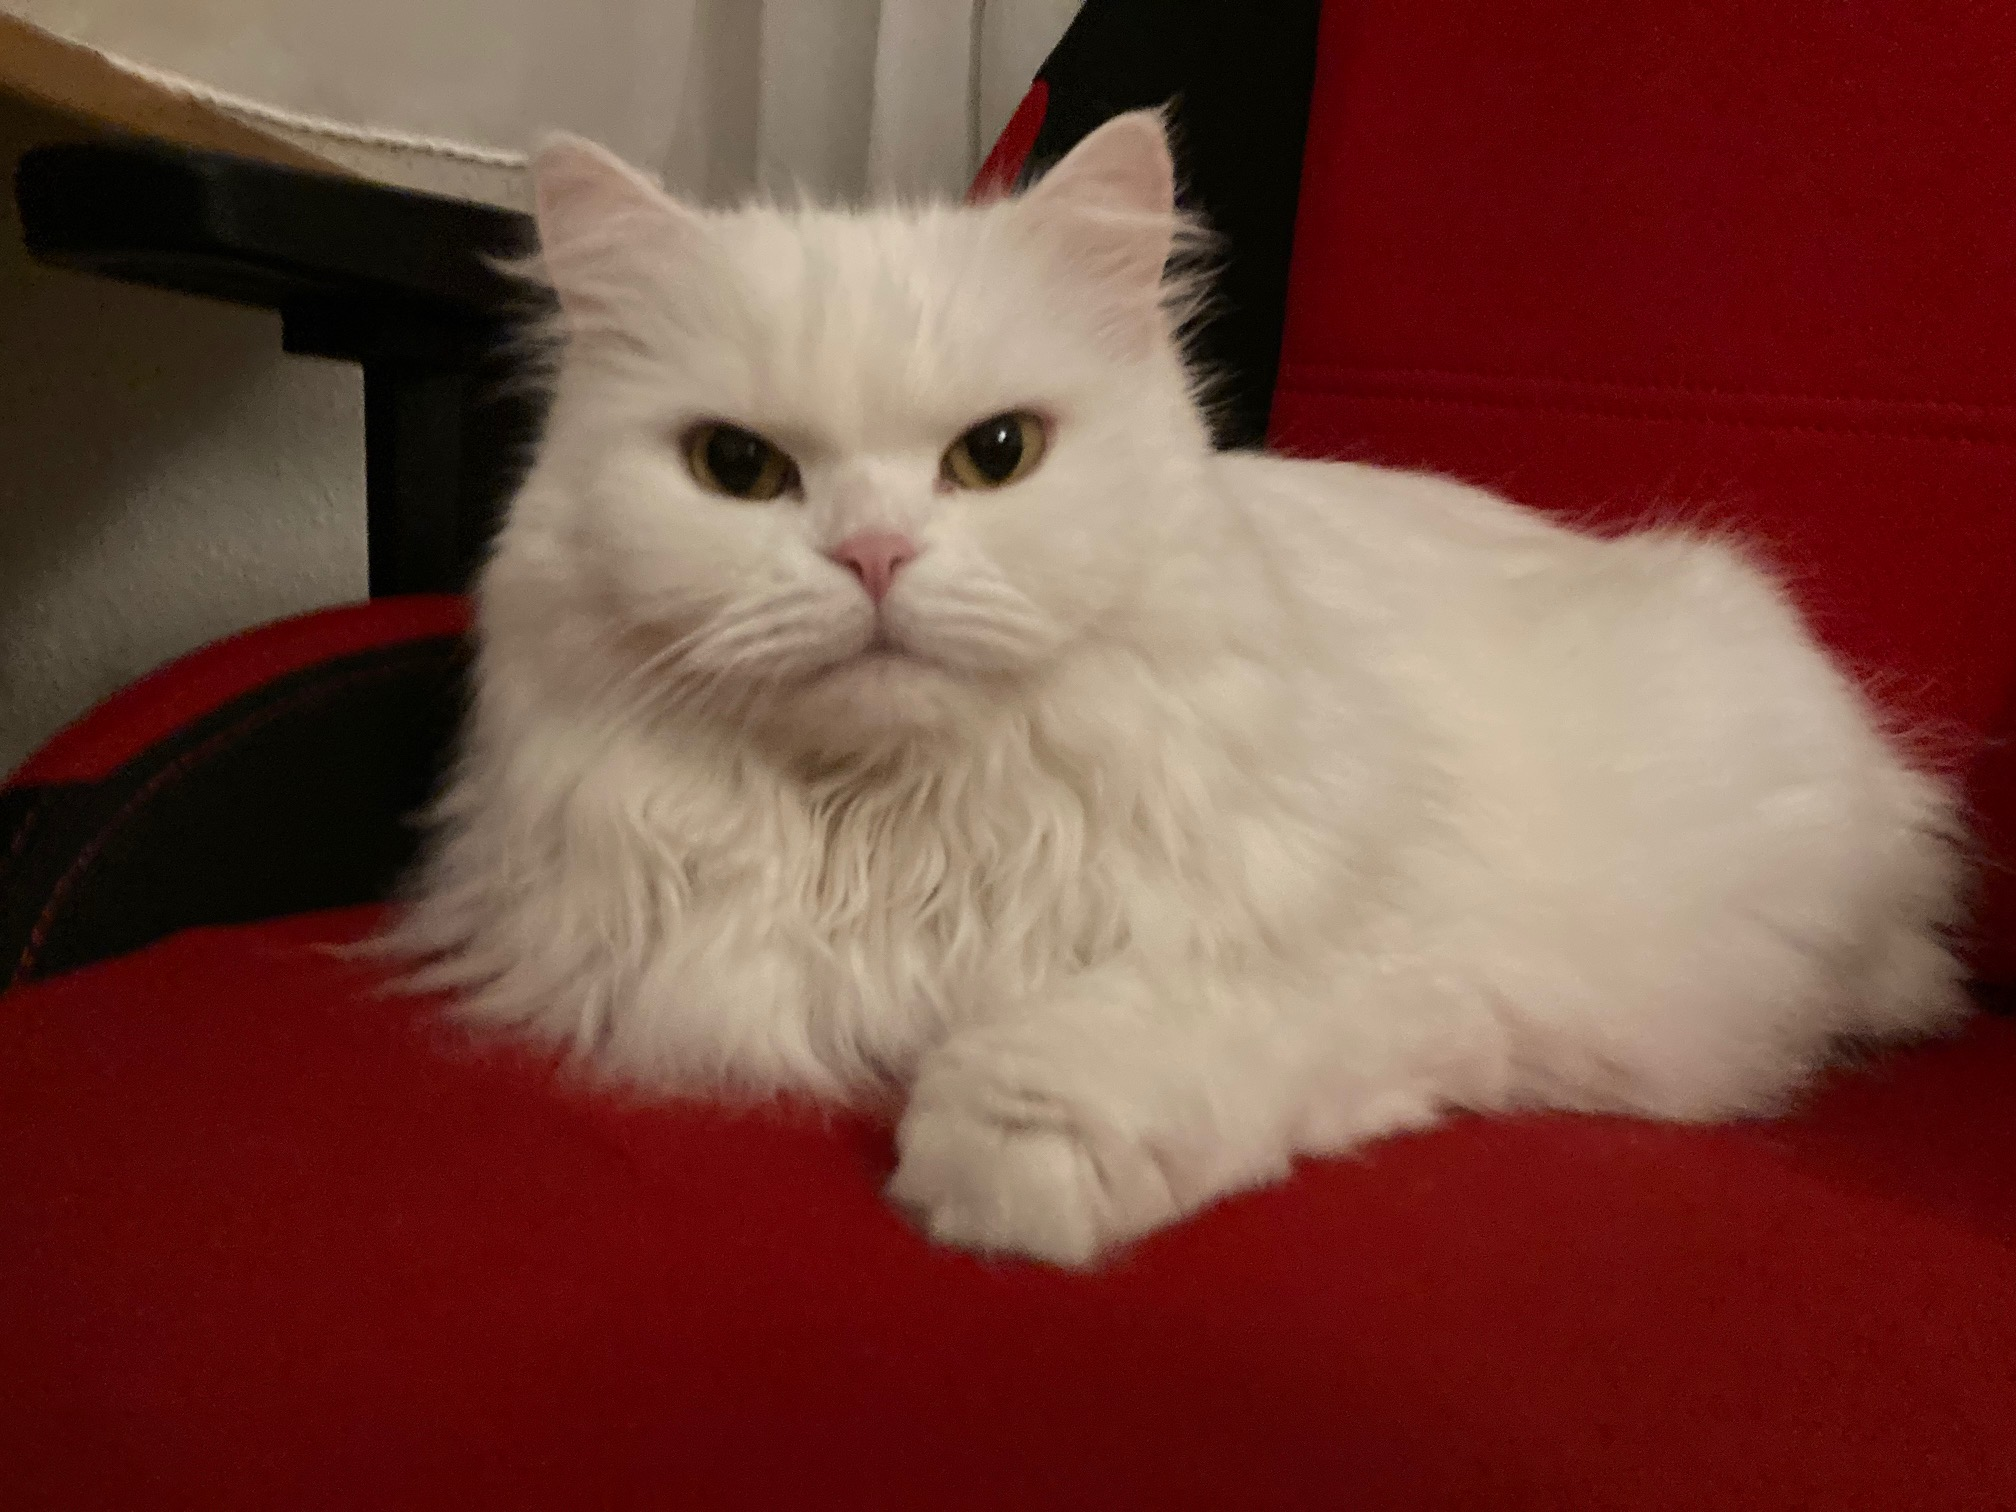
\includegraphics[width=\textwidth]{Bilder/Katze}
\caption{Meine Katze}\label{fig:Katze}
\end{figure}

\section{Blub}
\blindtext[5]

% Alternative zum Float
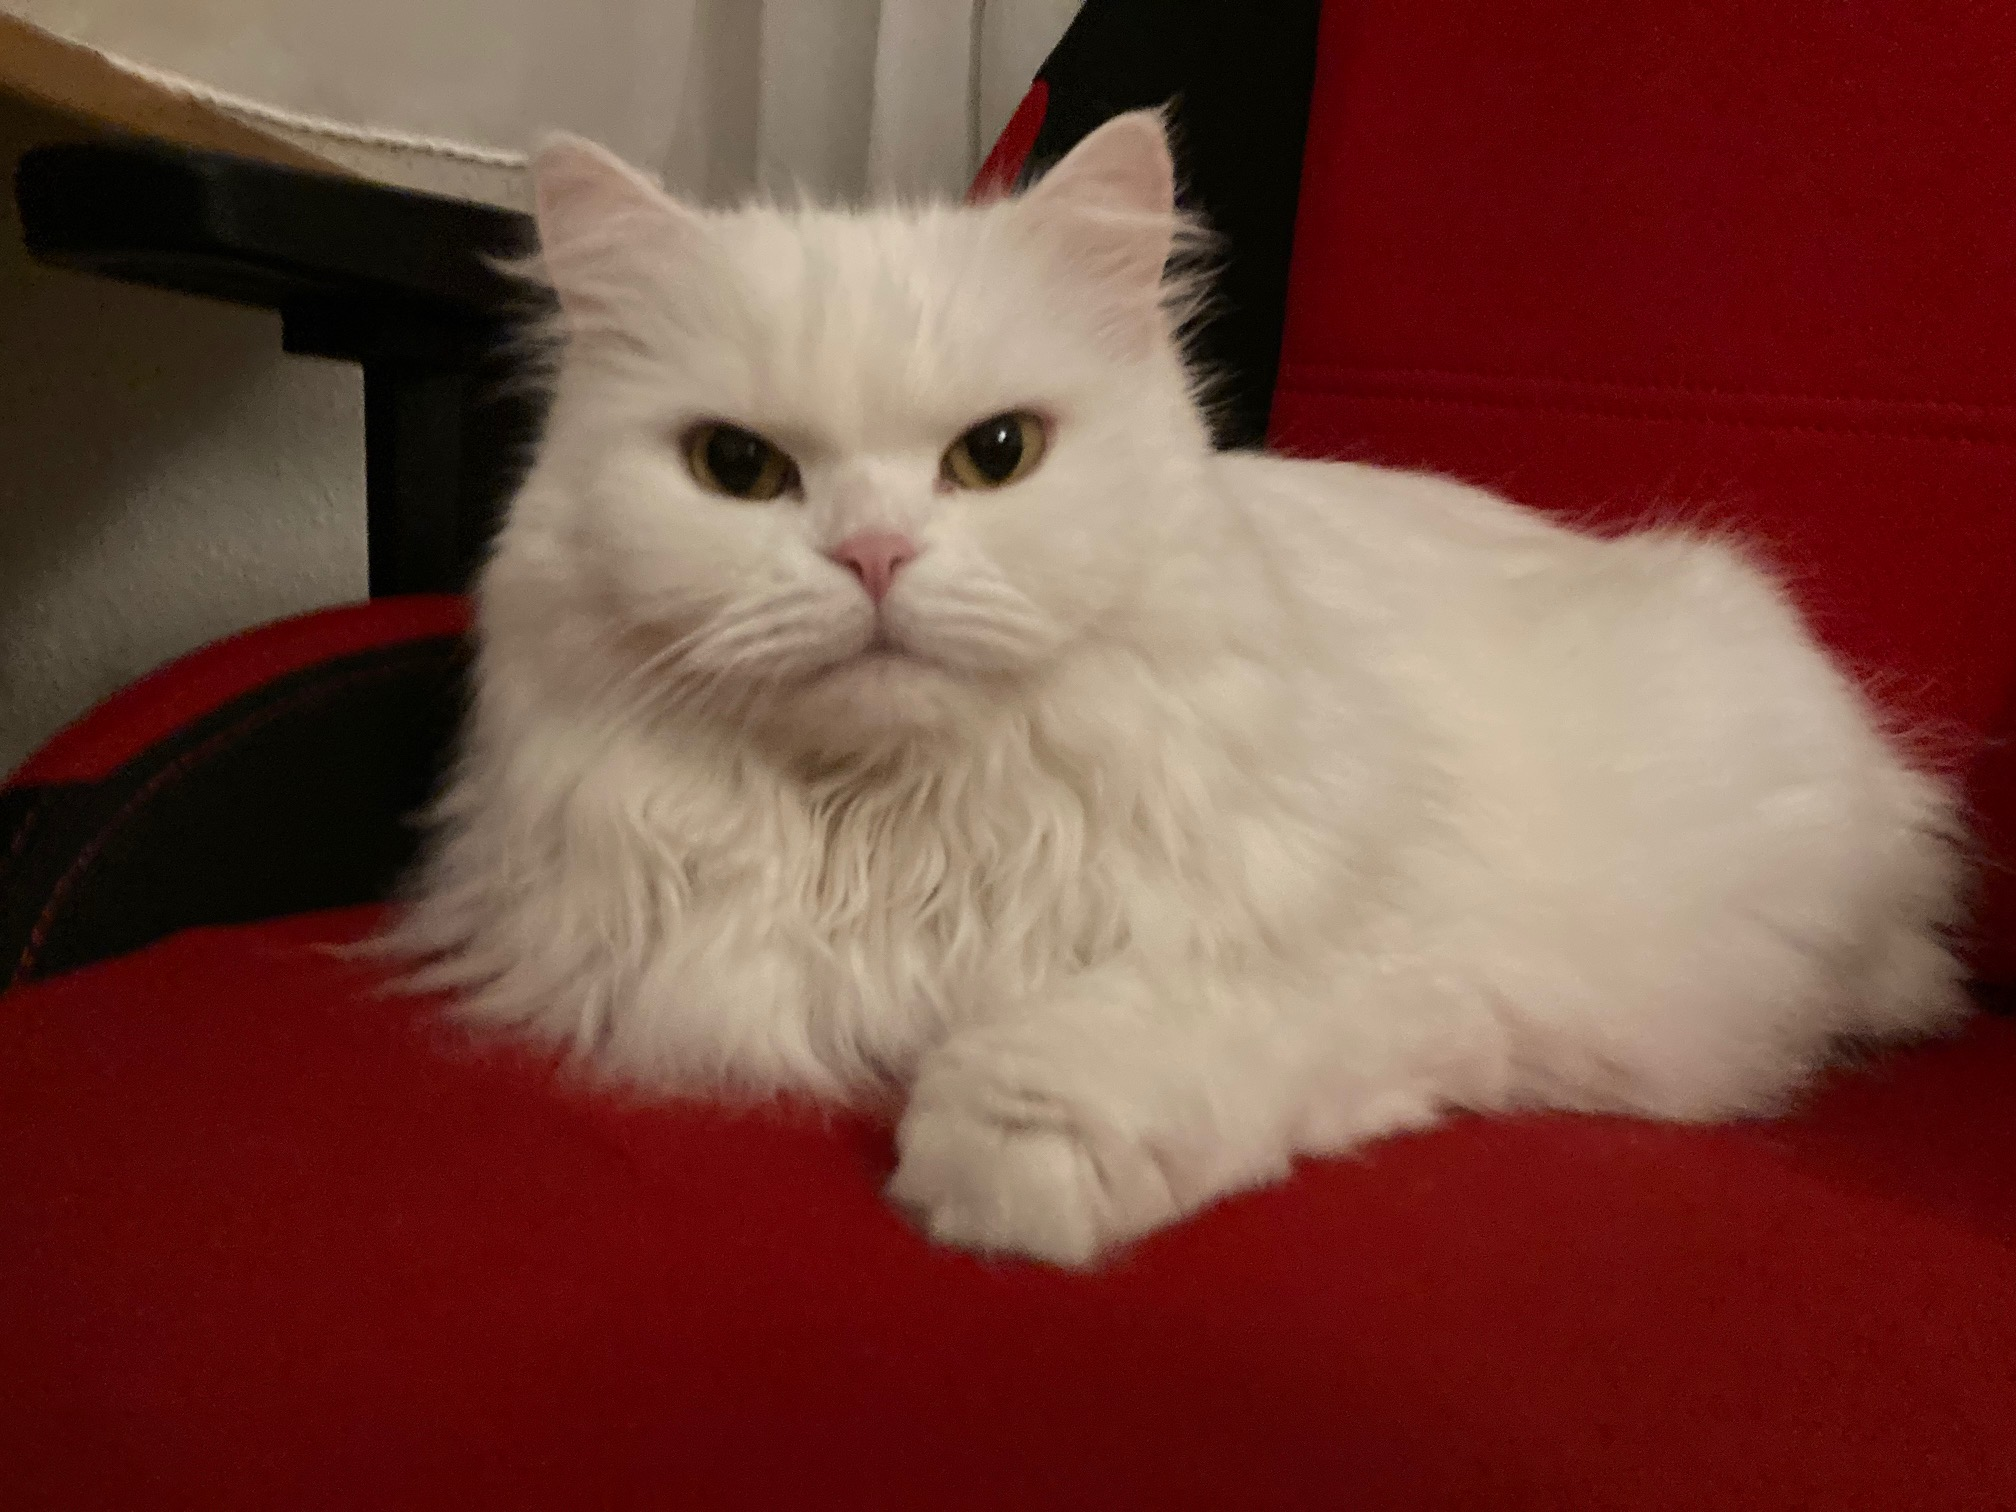
\includegraphics[width=\textwidth]{Bilder/Katze}
\captionof{figure}{Meine Katze 2}\label{fig:Katze2}

\blindtext[12]

\end{document}